\documentclass{article}

\usepackage[margin=1in]{geometry}
\usepackage{amsmath,amssymb}
%\usepackage{dsfont} %install texlive-fonts-extra 
\usepackage{tikz}
\usetikzlibrary{bayesnet}

\author{Otto Fabius}
\title{SGVB Topic Modelling}
\begin{document}

\maketitle

\section{Model}

We will consider the following graphical model:

\begin{figure}[ht]
  \begin{center}
    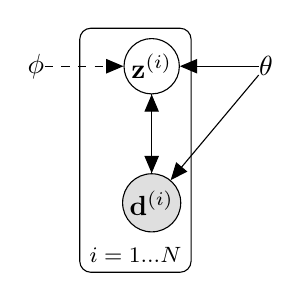
\begin{tikzpicture}[node distance = 1.5cm]
        \node[obs] (x) {$\mathbf{d}^{(i)}$}; 

        \node[latent, above=of x] (z) {$\mathbf{z}^{(i)}$}; 
        

        \node[const, right=of z] (th) {$\theta$} ;
        \node[const, left=of z] (ph) {$\phi$};

        \edge {z} {x};
        \edge {th} {z};
        \edge {th} {x};

        \edge [dashed] {ph} {z}
        \edge [dashed,bend left] {x} {z}

        \plate {xzd} {(x)(z)} {$i = 1...N$};

    \end{tikzpicture}
  \end{center}
\caption{Graphical Model. We have $N$ data points and both $z^{(i)}$ and $d^{(i)}$ are vectors}
\label{sgvb}
\end{figure}


In our application, $\mathbf{d}^{(i)}$ is a document (a vector of word frequencies), selected from the dataset containing N documents with uniform probability. The topic of each document $\mathbf{d}^{(i)}$ is represented by $k$ (continuous) latent variables $\mathbf{z}^{(ik)}$, with $p(\mathbf{z}^{(ik)}|\mathbf{d}^{(i)})$ a multivariate normal distribution with diagonal covariance. \\
We approximate the true posterior $p(z|d)$ by $q_\phi(z|d)$ parametrized by $\phi$, once again with $p(z|d)$ a multivariate normal distribution with diagonal covariance. The distributions $p_\theta(z|d)$ and $q_\phi(z|d)$ are neural networks, of which the parameters $\theta$ and $\phi$ are to be learned jointly. The output of $p_\theta(z|d)$ and $q_\phi(z|x,d)$ are the mean and the diagonal entries of the covariance matrix.

\section{Math}

\subsection{Lower Bound}

The log-likelihood of a data point i can be written as a sum of the lower bound and the KL divergence term between the true posterior $p(z|x,d)$ and the approximation $q(z|x,d)$, with $\theta$ the parameters of the model:

\begin{align*}
	\log p(\mathbf{d}^{(i)}) = D_{KL}(q(\mathbf{z}^{(i)}|\mathbf{d}^{(i)}) || p(\mathbf{z}|\mathbf{d}^{(i)})) + \mathcal{L}(\mathbf{\theta}, \phi)
\end{align*}

We optimize the lowerbound: 

\begin{align}
\mathcal{L}(\mathbf{\theta}, \phi; \mathbf{d}^{(i)}) = 
\mathbf{E}_{q_\phi (\mathbf{z}|\mathbf{d}^{(i)})}[-\log q_\phi (\mathbf{z}| \mathbf{d}^{(i)})+\log p_\theta(\mathbf{z}^{(i)}|\mathbf{d}^{(i)} ]
\end{align}

which, using Bayes rule, we can express as:

\begin{align}
\mathcal{L}(\mathbf{\theta}, \phi; \mathbf{d}^{(i)}) = -D_{KL}(q_\phi (\mathbf{z}| \mathbf{d}^{(i)})||q_\phi (\mathbf{z}| \mathbf{d}^{(i)})) + \mathbf{E}_{q_\phi(\mathbf{z}|\mathbf{d}^{(i)})}[\log p_\theta (\mathbf{d}^{(i)}|\mathbf{z})]
\end{align}


\subsection{KL Divergence}

We can integrate the KL divergence analytically. We don't use indices $^{(i)}$ for this integral. Further, $\mathbf{\mu}_\theta$ and $\mathbf{\sigma}_\theta^2$ represent the parametrized $p_\theta(\mathbf{z}|\mathbf{d})$.

Similar to Kingma and Welling\footnote{kingma} we obtain:

\begin{align}
- D_{KL}(q_\phi (\mathbf{z}| \mathbf{d})||p_\theta (\mathbf{z}| \mathbf{d})) = \frac{1}{2}\sum\limits_{j=1}^{J}\{1+\log \sigma_{\phi ,j}^2 - \mu_{\phi,j}^2 - \sigma_{\phi ,j}^2\}
\end{align}

\subsection{Final objective function}

We have a Poisson probability distribution on our outputs such that the reconstruction error becomes:

\begin{align}
\log p_{\theta}(y^{(i)}|d^{(i)}) = \sum_{k=1}^K\{-y^{(ik)} + d^{(ik)} \log{y^{(ik)}}\}
\end{align}
Where $k$ is the index of the output unit.\\


Using a SGVB estimator, our final objective function consists of the negative KL divergence (3) and the reconstruction error (4):

\begin{align}
\mathcal{L}(\mathbf{\theta}, \phi; \mathbf{x}^{(ik)},
 \mathbf{d}^{(i)}) = \sum_{k=1}^K\{-y^{(ik)} + d^{(ik)} \log{y^{(ik)}}\} + \sum_{k=1}^K\{-y^{(ik)} + d^{(ik)} \log{y^{(ik)}}\}
\end{align}
\end{document}